\begin{figure*}[t]
     \centering
     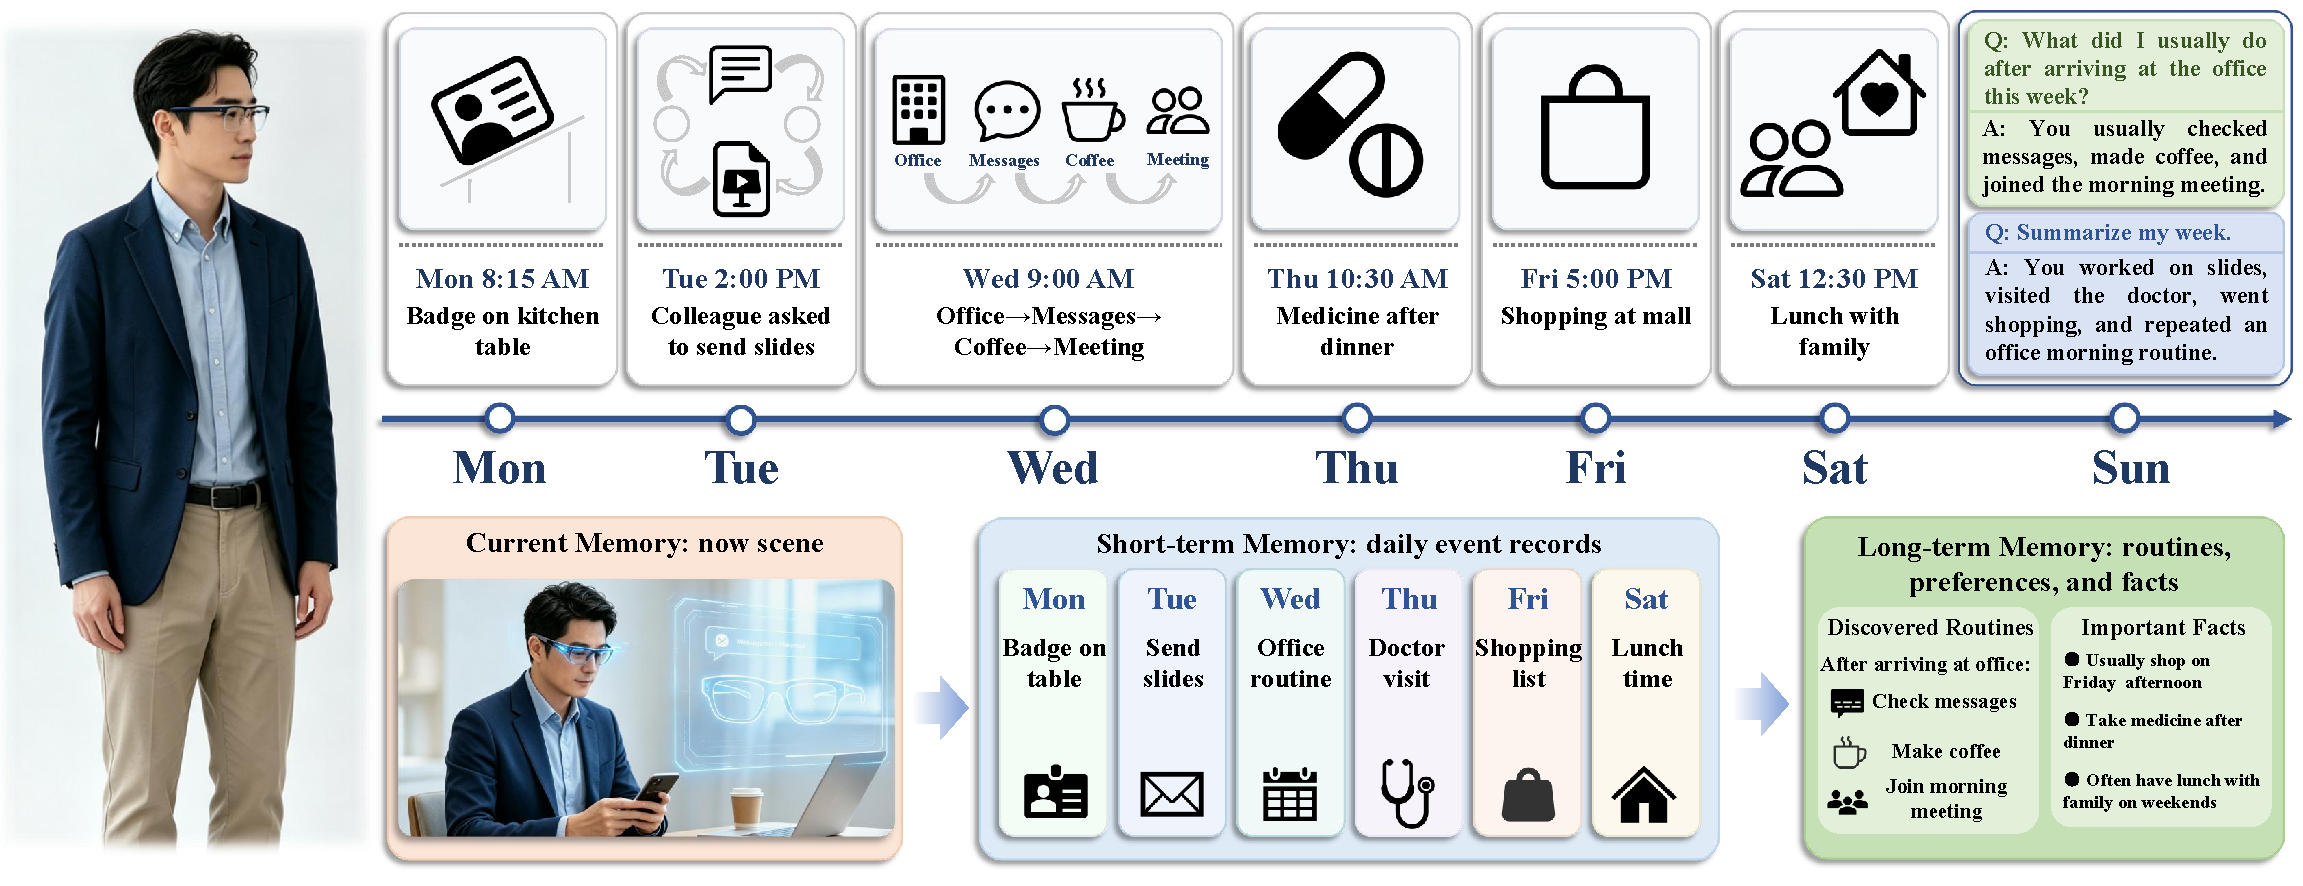
\includegraphics[width=\textwidth]{figures/case_new.pdf}
     \caption{
     Representative demonstration scenarios of \textbf{LightMem-Ego}. 
     The system supports immediate assistance, conversation recall, life summarization, 
     and routine discovery by retrieving evidence from hierarchical memory.
     }
     \label{fig:demo_scenarios}
     \vspace{-5mm}
\end{figure*}

\section{Demonstration}

Figure~\ref{fig:demo_scenarios} summarizes the main demonstration scenarios of LightMem-Ego. 
We organize the demo around everyday memory needs that span 
immediate scene understanding, recent event recall, and long-term routine reasoning.

\paragraph{Immediate Assistance.}
LightMem-Ego supports immediate assistance and short-horizon recall in mobile and AI-glasses settings. 
For example, users may ask \emph{Where did I leave my badge?}, \emph{When did I last hold my keys?}, or \emph{What am I looking at now?} 
In these cases, the system retrieves relevant recent observations and event segments, and returns answers grounded in temporally localized memory evidence. 
This case demonstrates how online perception and short-term memory can work together in everyday environments.

\paragraph{Conversation Recall.}
LightMem-Ego also supports recall of recent spoken interactions. 
After a meeting or conversation, users can ask questions such as \emph{What did the doctor tell me after checking the report?} or \emph{What did my colleague ask me to do?} 
The system combines short-term event memory with aligned transcript context to recover the relevant conversational episode. 
This shows the value of multimodal memory for recovering spoken information beyond one-shot speech transcription.

\paragraph{Life Summarization and Routine Discovery.}
Beyond recovering isolated facts, LightMem-Ego can summarize recent experiences and reason over repeated patterns. 
A user may ask \emph{What did I do this afternoon?}, \emph{Summarize what happened during lunch}, or \emph{What do I usually do after arriving at the office?} 
The system aggregates event-centered evidence across multiple segments and, when appropriate, draws on long-term semantic memory to identify recurring activities, preferences, and routines. 
This scenario illustrates the ability of LightMem-Ego to move from event recall to higher-level summarization and habit-level reasoning.